\documentclass[titlepage]{article}
 \usepackage[utf8]{inputenc}
\usepackage{listings}
\usepackage{amsmath}
\usepackage{float}
\usepackage{verbatim} 	
\usepackage{graphicx}
\graphicspath{ {imagenes/} }
 \usepackage{xcolor}
 \definecolor{RoyalBlue}{cmyk}{1, 0.50, 0, 0}

\lstset{language=Java,
	keywordstyle=\color{RoyalBlue},
	basicstyle=\scriptsize\ttfamily,
	commentstyle=\ttfamily\itshape\color{gray},
	stringstyle=\ttfamily,
	showstringspaces=false,
	breaklines=true,
	frameround=ffff,
	frame=single,
	rulecolor=\color{black}}


 

% Datos de la portada
\begin{document}
	\begin{titlepage}
		\begin{center}
			\vspace*{1cm}
			\date{} % para que no aparezca la fecha la dejo en blanco
			\Huge
			\textbf{Cuestionario 3}
			
			\vspace{0.5cm}
			\LARGE
			Aprendizaje Automático
			
			\vspace{1.5cm}
			
			\textbf{José Manuel Pérez Lendínez}
			

			
		\end{center}
	\end{titlepage}	
	\newpage

\section{Podría considerarse Bagging como una técnica para estimar el error de predicción de un modelo de aprendizaje?. Diga si o no con argumentos. En caso afirmativo compárela con validación cruzada.}
	
Si, puesto que ajusten de forma repetida empleando muestras generadas por bootstrapping conlleva a que, en promedio, cada ajuste usa solo aproximadamente dos tercios de las observaciones originales. Al tercio restante se le llama out-of-bag (OOB). Si para cada árbol ajustado en el proceso de bagging se registran las observaciones empleadas, se puede predecir la respuesta de la observación i haciendo uso de aquellos árboles en los que esa observación ha sido excluida (OOB) y promediándolos (la moda en el caso de los árboles de clasificación). Por tanto con ese proceso podemos estimar el error para las n observaciones. Como se utilizan solo los arboles que no participo la observación i, podemos considerar esta estimación como el test-error. 

En validación cruzada se parten los datos en n particiones. Se n-1 particiones para el train y 1 para el test y se repite este proceso cambiando la partición de test por otra en cada iteración hasta que todas las particiones han pasado por el test. Se obtiene la aproximación del error como la media de los errores de todas las interacciones.
  
En bagging en cambio utiliza muestreo repetido para reducir la varianza. Utiliza bootstrapping para realizar nuevas muestras del mismo tamaño con repeticiones y dejando fuera una parte de ellas que se utilizara para predecir (OOB). En este caso se utilizada distintos modelos de predicción para cada partición y promediamos las predicciones resultantes.
  	 
\section{Considere que dispone de un conjunto de datos linealmente separable. Recuerde que una vez establecido un orden sobre los datos, el algoritmo perceptron encuentra un hiperplano separador interando sobre los datos y adaptando los pesos de acuerdo al algoritmo}
\begin{figure}[H]
	\centering
	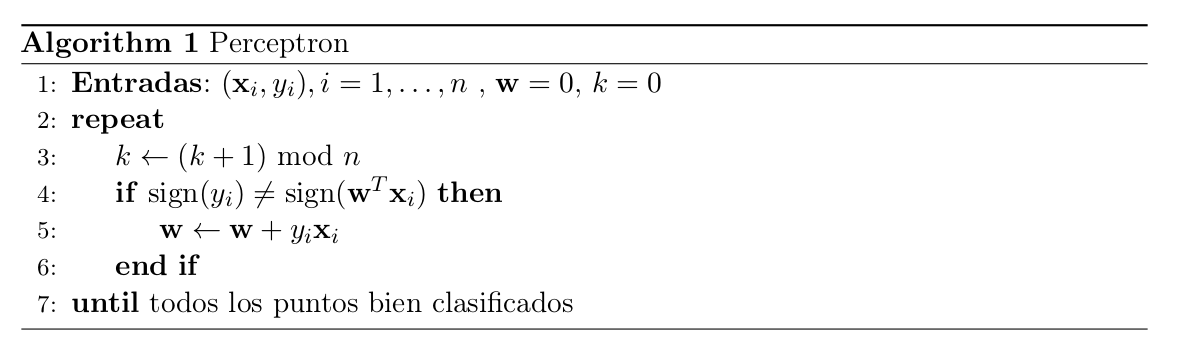
\includegraphics[width=1\linewidth]{screenshot005}
	\caption{}
	\label{fig:screenshot005}
\end{figure}
\newpage
\section{Considerar un modelo SVM y los siguientes datos de entrada: Clase-1{(1,1),(2,2),(2,0)}, Clase-2:{(0,0),(1,0),(0,1)}}.

\begin{enumerate}
	\item Dibujar los puntos y construir por inspección el vector de pesos para el hiperplano óptimo y el margen óptimo.
	Se ve muy facilmente cual seria el hiperplano optimos que caeria en la funcion y = 1.5 - x (linea roja). Los margen optimos(lineas negras) se marcan por las funciones y = 1 - x y la funcion y = 2 - x
		\begin{figure}[H]
			\centering
			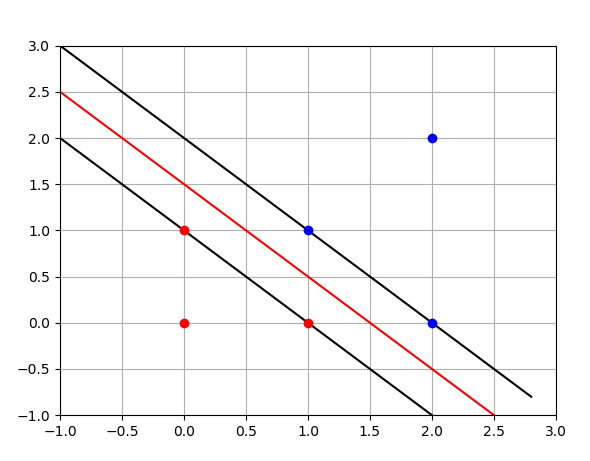
\includegraphics[width=0.7\linewidth]{screenshot003}
			
		\end{figure}

	\newpage
	\item ¿Cúales son los vectores soporte?
	\begin{figure}[H]
		\centering
		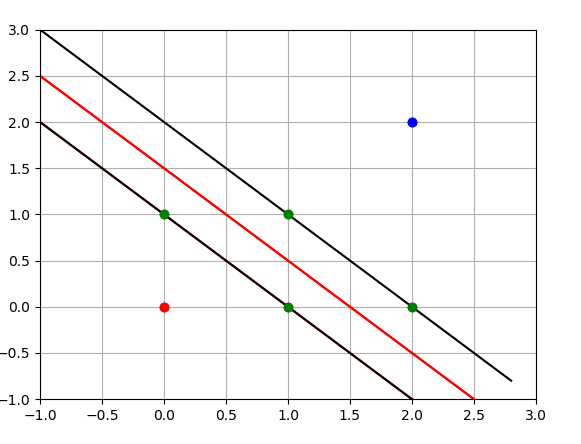
\includegraphics[width=0.7\linewidth]{screenshot002}

	\end{figure}
	Los cuatro puntos que que caen sobre la lineas de margen son los vectores soporte.

	\item Construir la solución en el espacio dual. Comparar la solución con la del apartado (a)

\end{enumerate}

\section{¿Cúal es el criterio de optimalidad en la construcción de un árbol? Analice un clasificador en árbol en términos de sesgo y varianza. ¿Que estrategia de mejora propondría?}

\section{¿Como influye la dimensión del vector de entrada en los modelos: SVM, RF, Boosting and NN}

\begin{enumerate}
	\item SVM: En este caso la dimensión del vector de datos no tiene una gran influye en el modelo puesto que lo que utilizan es la distancia entre los cada vector de entrada. De esta manera si se tiene 10 vectores de entrada no importa si el vector de datos tiene 10 o 1000 entrada. Solo tendremos en cuenta que tendremos n/(n-10)/2 distancias. En este caso serian 45 distancias.
	
	\item Random forest: En este caso para cada arbolo se utilizaran un numero de variables de el vector de entrada y no todas ellas para entrenarse. Se tendrán varios arboles trabajando cada uno con un conjunto de variables elegidas aleatoriamente. Lo único que tendremos que tener en cuenta es elegir un numero de variables con el que trabajaran todos los arboles y el numero de arboles necesarios para que se pueda trabajar con todas las variables y se puedan obtener información importante de la relación que tienen cada variable. Esto los hace buenos para grandes dimensionalidad de datos.
\end{enumerate}

\section{El método de Boosting representa una forma alternativa en la búsqueda del mejor clasificador respecto del enfoque tradicional implementado por los algoritmos PLA, SVM, NN, etc. 1) Identifique de forma clara y concisa las novedades del enfoque; 2) Diga las razones profundas por las que la técnica funciona produciendo buenos ajustes (no ponga el algoritmo); 3) Identifique sus principales debilidades; 4) ¿Cuál es su capacidad de generalización comparado con SVM?}
\begin{enumerate}
	\item{Identifique de forma clara y concisa las novedades del enfoque:}  Se trabaja siempre con el conjunto completo de entrada, y se manipulan los pesos de los datos para generar modelos distintos. Se le da mas pesos a los datos mal clasificados. Utilizando clasificadores sencillos. Cada clasificador utilizara los datos del clasificador anterior.
	
	\item{ Identifique sus principales debilidades:} Su principal debilidad viene dada por el ruido. Al darle mayor importancia a los datos mal clasificados si le podríamos estar dando importancia a un dato erroneo y no podríamos saberlo. O el caso contrario un dato que creemos bien clasificado no lo esta. Esto se ha demostrado que con conjunto de datos con ruido, esta técnica no funciona nada bien.
\end{enumerate}
\section{Discuta pros y contras de los clasificadores SVM y Random Forest. Considere que SVM por su construcción a través de un problema de optimización debería ser mejor clasificador que RF. Justificar las respuesta.}

\textbf{SVM:}
\begin{enumerate}
	\item Pros
	\begin{enumerate}
		\item Para calcular la frontera solo necesitara los vectores de soporte al calcularse el hiperplano solo atraves de estos. Al utilizar distancias no le afecta tanto la dimensionalidad de los vectores y es bueno para datos con gran dimensionalidad.
		\item Si el modelo es lineal-mente separable y no tiene ruido obtendrá el optimo. Ya que se quedara el hiperplano que de la mayor distancia posible de los vectores de soporte.
		\item Utilización de núcleo para utilizar transformaciones no lineales.
	\end{enumerate}
	\item Contras
	\begin{enumerate}
		\item Para problemas multiclase se tendría que utilizar métodos como one vs rest. Complicando el modelo. 
		\item Si se elige un mal núcleo el modelo puede empeorar mucho. Esto podría realizar un sobre ajuste demasiado fuerte.
		\item Es algo pero con variables categóricas que con numéricas.
		
	\end{enumerate}
\end{enumerate}

\textbf{RF:}
\begin{enumerate}
	\item Pros
	\begin{enumerate}
		\item Si tiene una gran cantidad de datos seria uno de los mejores algoritmos a utilizar. Siendo muy eficiente para grandes cantidades de datos. Se adapta también muy bien a grandes cantidades de variables para una entrada.
		
		\item Es capaz de detectar las variables mas importantes de nuestros datos y las interacciones entre variables. 
		
		\item Mejora el rendimiento de los modelos lineales en modelos no lineales.
		
		
	\end{enumerate}
	\item Contras
	\begin{enumerate}
		\item Si el conjunto de datos tiene ruido puede afectar mucho al rendimiento de RF.
		\item Es complicado de interpretar al utilizar la combinación de muchos arboles distintos
	\end{enumerate}
\end{enumerate}

No se puede asegurar que SVM clasifique siempre mejor que RF, debido a que por ejemplo con una gran cantidad de datos RF seria mucho mas eficiente y rápido que SVM. También podría ser mejor RF en datos con muchas variables categóricas. Otro caso en el que RF podría ser mejor que SVM seria en funciones no lineales, ya que para este tipo de funciones SVM dependerá mucho del kernel utilizado.

\section{¿Cuál es a su criterio lo que permite a clasificadores como Random Forest basados en un conjunto de clasificadores simples aprender de forma mas eficiente? ¿Cuales son las mejoras que introduce frente a los clasificadores simples? ¿Es Random Forest óptimo en algún sentido?}

\begin{enumerate}
	\item \textbf{¿Cuál es a su criterio lo que permite a clasificadores como Random Forest basados en un conjunto de clasificadores simples aprender de forma mas eficiente?}
	
	En este caso creo que es debido a la utilización de muchos clasificadores simples y a partir de estos forma el clasificador final. Esto es debido a que a la hora de realizar la separación de datos reduce la varianza de estos y como no trabaja con todas las variables tampoco en cada clasificador simple es capaz de encontrar variables mas útiles. Por tanto con un bueno numero de arboles y una buena cantidad variables utilizada en cada árbol se podría tender en cuenta muchos casos mas individualmente que los métodos que utilizan un único modelo de clasificar no podrán tener en cuenta.
	
	\item \textbf{¿Cuales son las mejoras que introduce frente a los clasificadores simples?}
	La mejora es que utiliza varios clasificadores simples (uno por arbol) en vez de un único clasificador simple. Esto unido a que a cada árbol le asigna un conjunto de datos distinto con varianzas semejantes y un conjunto de variables distintos para analizar, esta clasificando los datos de formas distinta en cada árbol, quedándose en cada árbol con distintas características de los datos que pueden ser buenas para clasificarlos. Por esto al unir después las predicciones de todos los clasificadores, pueden ser menos genéricas y tener en cuenta distintos escenarios que con un único clasificador simple seria imposible.
	
	\item \textbf{¿Es Random Forest óptimo en algún sentido?}
	Random Forest lo podríamos tener como un modelo optimo cuando tenemos un gran conjunto de datos con vectores de gran dimensionalidad y sabemos que nuestros datos no contiene ruido. Debido a que es muy eficiente al trabajar en cada clasificador solo con un conjuntos de variables y no con todas y al tener muchos datos podremos explorar escenarios muy distintos con clasificadores simples que nos hará tener mucha información del problema. Aunque como utiliza en la división de los datos y las variables aleatoriedad no se podría nombra como optimo.
	
\end{enumerate}

\section{En un experimento para determinar la distribución del tamaño de los peces en un lago, se decide echar una red para capturar una muestra representativa. Así se hace y se obtiene una muestra suficientemente grande de la que se pueden obtener conclusiones estadísticas sobre los peces del lago. Se obtiene la distribución de peces por tamaño y se entregan las conclusiones. Discuta si las conclusiones obtenidas servirán para el objetivo que se persigue e identifique si hay algo que lo impida.}
No. Esto se debe a la forma de seleccionar la poblacion de nuestra muestra. Si solo realizamos un único lanzamiento de la red en todo el lago solo podremos ser capaces de tener una muestra representativa de esa única zona. Si en esa zona solo vivieran peces de una especie esa muestra no seria validad para toda la poblacion del lago. Quizas se tendría que realizar el lanzamiento de la red en distintas zonas del lago y a distintas profundidades. 

\section{Identifique que pasos daría y en que orden para conseguir con el menor esfuerzo posible un buen modelo de red neuronal a partir una muestra de datos. Justifique los pasos propuestos, el orden de los mismos y argumente que son adecuados para conseguir un buen óptimo. Considere que tiene suficientes datos tanto para el ajuste como para el test.}

En este caso solo necesitaremos dos pasos:
\begin{enumerate}
	\item Inicializar pesos: Para esto tendremos que tener en cuenta que si se inicializan a a cero o a un mismo valor llegaríamos a un optimo local. Si se inicializan a valores muy altos se satura la función sigmoidal se saturaría. Lo mas recomendables es inicalizarlo con valores cercanos a cero mediante una distribución normal .
	
	\item Criterio de terminación: Si no conseguimos un buen criterio de parada podrian darse el caso de que el algoritmo nunca lo alcance y no llegue a parar nunca o el caso contrario que seria una parada prematura antes de llegar a un buen modelo. En este caso los parametros que podríamos tener en cuenta en el criterio de parada podrian ser:
	\begin{enumerate}
		\item Maximo de iteraciones
		\item Tamaño del gradiente.
	\end{enumerate}

	Se podrían mezclar varios de estos criterios.
\end{enumerate}
  	
  	
\end{document}